\chapter{Interrogazione dell'ontologia}
Questo capitolo esplora dettagliatamente le regole SWRL e le query SPARQL sviluppate durante il progetto, illustrando come queste tecniche siano state implementate per arricchire la fruibilità dell'ontologia.\\

Le regole SWRL forniscono un meccanismo potente per inferire nuove conoscenze all'interno dell'ontologia, consentendo di dedurre informazioni aggiuntive sulla base delle relazioni e delle proprietà definite. Questo strumento si è rivelato fondamentale per estendere la completezza dell'ontologia e fornire una visione più approfondita del dominio. Mentre, le query SPARQL rappresentano uno strumento essenziale per recuperare informazioni specifiche dall'ontologia. Attraverso l'utilizzo di SPARQL, è possibile eseguire interrogazioni complesse che permettono di individuare istanze specifiche dall'ontologia.

\section{SWRL}\label{sec:swrl}
All'interno di questa sezione, ci dedicheremo all'analisi delle regole SWRL, che sono state integrate nell'ontologia BDOnto. Queste regole sono state concepite con l'obiettivo di inferire nuove informazioni o di assegnare classificazioni alle istanze presenti nell'ontologia in base a specifiche condizioni. Ciascuna di queste regole svolge un ruolo distintivo all'interno del complesso processo di arricchimento dell'ontologia.\\

In totale sono state create 5 regole SWRL, che permettono di calcolare:
\begin{itemize}
    \item \texttt{BDOnto - Server Definition}: identifica quali istanze di Desktop possono essere anche Server in base ad alcune caratteristiche: il computer deve avere almeno una CPU con frequenza di Clock di 3 GHz, 8 GB di RAM e 500 GB di disco fisico.
    \item \texttt{BDOnto - Server Enterprise Definition}: identifica quali istanze di Desktop possono essere anche Server Enterprise in base ad alcune caratteristiche: il computer deve avere almeno una CPU con frequenza di Clock di 3 GHz, 8 GB di RAM, 500 GB di disco fisico e una GPU con 2 GB di memoria dedicata.
    \item \texttt{BDOnto - hasPlatform Definition}: stabilisce quale è la piattaforma/compagnia che si occupa di una data tecnologia sulla base del suo nome completo.
    \item \texttt{BDOnto - hasVersion Definition}: stablisce quale sia la versione di una tecnologia sulla base del nome completo.
    \item \texttt{BDOnto - hasLifespan Definition}: si calcola per quanti mesi una tecnologia è stata supportata.
\end{itemize}

\subsection{Premessa}\label{subsec:premswrl}
Data la natura del linguaggio SWRL alcune regole che avremmo voluto sviluppare non sono state possibili. Ad esempio, avremmo voluto creare una interrogazione che comprendesse una negazione. La negazione, a causa del principio di monotonicità che implica che una volta che si acquisiscono nuove informazioni, queste non vengono negate o rimosse, non è ammessa in SWRL.\\

Inoltre, volevamo utilizzare SWRL per estrapolare informazioni di diversa natura (es. la durata totale del supporto ad una tecnologia) e, tramite questo percorso, approfondire le nostre conoscenze a riguardo. In un primo momento è stata effettuata un'analisi di come avremmo potuto implementare queste regole. Dalle prime ricerche abbiamo individuato le Built-Ins per le date, definite dal W3C \cite{datetime_builtin} e la SWRL Temporal Built-In Library \cite{SWRLTemporalBuiltInsBasic}. I problemi con la prima soluzione sono nati in fase di reasoning. Infatti il reasoner utilizzato da noi, e maggiormente consigliato Pellet \cite{pelletreasoner}, supporta solo le prime 5 built-ins temporali del W3C \cite{datetime_builtin} (si veda \cite{pelletsupporttime}): ne risultava una scarsa "potenza" di approfondimento delle informazioni. Siamo poi passati all'impiego della libreria \texttt{temporal} \cite{SWRLTemporalBuiltInsBasic}. Dopo tanti tentativi, siamo riusciti ad utilizzarla a dovere e a costruire una regola che impiegasse tale costrutto \ref{subsec:haslifespan}.\\

Alcune piccole note tecniche. Nel caso in cui, anche dopo aver fatto partire il reasoner, alcune data properties che dovrebbero essere inferite non vengono mostrate a schermo, probabilmente non avete spuntato la casella per la visualizzazione di tali proprietà. Poi, nell'interfaccia principale di Protègè, bisogna andare in \texttt{Reasoner -> Configure -> Displayed inferences} e spuntare tutte le caselle relative alle data properties. Inoltre, il reasoner Pellet non supporta la libreria \texttt{temporal} \cite{SWRLTemporalBuiltInsBasic}, quindi per ottenere le informazioni relative al lifespan contenute in \ref{subsec:haslifespan} si deve:
\begin{itemize}
    \item Aprire una tab per il plugin SWRLTab;
    \item Cliccare il bottone \texttt{OWL+SWRL->Drools} e aspettare che termini;
    \item Cliccare il bottone \texttt{Run Drools} e aspettare che termini;
    \item A questo punto le informazioni sono state inferite ma ancora non vengono mostrate. Per mostrarle a schermo dobbiamo cliccare \texttt{Drools->OWL}. Facendo ciò molte informazioni verranno nuovamente aggiunte alla ontologia in maniera permanente. Se si vuole lasciare l'ontologia "pulita" è importante \textbf{non} salvare dopo aver fatto questo ultimo passaggio. Per ulteriori informazioni si faccia riferimento alla documentazione ufficiale del plugin \cite{SWRLTabplugin}.
\end{itemize}
Può capitare che la prima volta che si apre il file dell'ontologia all'interno di Protègè, e si ripete il processo definitio qui sopra per inferire le regole SWRL, vengano restituiti degli errori. Se per esempio viene rilevato un errore sulla regola \texttt{hasVersion}, copiare e incollare la regola definita in questo documento all'interno della regola definita in Protègè, salvare il file e poi ricaricare Protègè (\texttt{File -> Reload}). A questo punto l'errore dovrebbe scomparire.\\

Infine, nelle regole SWRL che mostriamo viene spesso ripetuta il predicato \texttt{swrlb:stringConcat}. Tale predicato è una sorta di soluzione alternativa al type conversion. Infatti, durante la realizzazione di queste regole SWRL, che dovevano funzionare in maniera uguale sia sul reasoner Pellet che sul reasoner del plugin SWRLTab, si sono affrontati spesso degli errori di conversione (es. \textit{cannot convert value of type PlainLiteral to xsd:string}). Il costo per la buona riuscita di tali regole in entrambi gli ambienti è stato l'incremento di complessità dato dall'aggiunta di tale predicato.\\

I tool impiegati in questa fase sono stati \textbf{Protègè} \cite{protegehomepage} ed il suo plugin \textbf{SWRLTab} \cite{SWRLTabplugin}.
\newpage 
\subsection{Server}
Questa regola è stata definita per meglio classificare quelle istanze di un computer che equivalgono ad una istanza di un server. Chiaramente alcune proprietà devono essere soddisfatte come la potenza della CPU (almeno 3 GHz di frequenza), la capacità della RAM (almeno 8 GB) e la disponibilità di memoria (almeno 500 GB). Di seguito la regola SWRL creata.\\

\begin{lstlisting}[language=Prolog]
Desktop(?d) ^
   cpuSpeedUnit(?d, ?us) ^ 
   cpuSpeedValue(?d, ?vs) ^
   deviceRAMUnit(?d, ?uc) ^
   deviceRAMValue(?d, ?vc) ^
   deviceStorageUnit(?d, ?ud) ^
   deviceStorageValue(?d, ?vd) ^
   swrlb:stringConcat(?sus, ""^^rdf:PlainLiteral, ?us)
   swrlb:stringEqualIgnoreCase(?sus, "GHz") ^
   swrlb:greaterThanOrEqual(?vs, 3.0) ^
   swrlb:stringConcat(?suc, ""^^rdf:PlainLiteral, ?uc)
   swrlb:stringEqualIgnoreCase(?suc, "GB") ^
   swrlb:greaterThanOrEqual(?vc, 8) ^
   swrlb:stringConcat(?sud, ""^^rdf:PlainLiteral, ?ud)
   swrlb:stringEqualIgnoreCase(?sud, "GB") ^
   swrlb:greaterThanOrEqual(?vd, 500) ->
   Server(?d)
\end{lstlisting}
\newpage
\subsection{Server Enterprise}
Questa regola, che risulta essere una estensione della precedente, definisce come classificare quei Desktop che hanno caratteristiche comuni ad i server enterprise. Le proprietà che devono rispettare sono le stesse dei server classici, con l'aggiunta di una GPU con almeno 2 GB di memoria dedicata. Di seguito la regola SWRL creata.\\

\begin{lstlisting}[language=Prolog]
Desktop(?d) ^
   hasGPU(?d, ?gpu) ^
   gpuMemoryUnit(?d, ?ug) ^
   gpuMemorySize(?d, ?vg) ^		
   cpuSpeedUnit(?d, ?us) ^ 
   cpuSpeedValue(?d, ?vs) ^
   deviceRAMUnit(?d, ?uc) ^
   deviceRAMValue(?d, ?vc) ^
   deviceStorageUnit(?d, ?ud) ^
   deviceStorageValue(?d, ?vd) ^
   swrlb:stringConcat(?sus, ""^^rdf:PlainLiteral, ?us)
   swrlb:stringEqualIgnoreCase(?sus, "GHz") ^
   swrlb:greaterThanOrEqual(?vs, 3.0) ^
   swrlb:stringConcat(?suc, ""^^rdf:PlainLiteral, ?uc)
   swrlb:stringEqualIgnoreCase(?suc, "GB") ^
   swrlb:greaterThanOrEqual(?vc, 8) ^
   swrlb:stringConcat(?sud, ""^^rdf:PlainLiteral, ?ud)
   swrlb:stringEqualIgnoreCase(?sud, "GB") ^
   swrlb:greaterThanOrEqual(?vd, 500) ^
   swrlb:stringConcat(?sug, ""^^rdf:PlainLiteral, ?ug)
   swrlb:stringEqualIgnoreCase(?sug, "GB") ^
   swrlb:greaterThanOrEqual(?vg, 2) ->
   Server_Enterprise(?d)
\end{lstlisting}
\newpage
\subsection{hasPlatform}
Questa regola serve ad associare una azienda ad una tecnologia. La motivazione di tale regola risiede nel fatto che può essere ripetitivo scrivere a quale compagnia è associato un certo prodotto. L'obiettivo è quindi quello di estrapolare dalle proprietà già definite all'interno di una istanza di \textit{Big\_Data\_Technology} questa informazione. E lo fa prima, estraendo il nome completo della tecnologia e di una azienda (\textit{Company}), successivamente, confronta se il nome completo della tecnologia contiene il nome completo della compagnia (ignorando le differenze tra maiuscole e minuscole) ed infine, se questa condizione è soddisfatta, la regola crea un collegamento tra le due istanze assegnando loro la proprietà \textbf{hasPlatform}. Di seguito la regola SWRL creata.\\

\begin{lstlisting}[language=Prolog]
Big_Data_Technology(?d) ^ 
   hasFullName(?d, ?dname) ^ 
   Company(?c) ^
   companyName(?c, ?cname) ^
   swrlb:stringConcat(?ddname, ""^^xsd:string, ?dname) ^
   swrlb:stringConcat(?dcname, ""^^xsd:string, ?cname) ^
   swrlb:containsIgnoreCase(?ddname, ?dcname) -> hasPlatform(?d, ?c)
\end{lstlisting}

\subsection{hasVersion}
Questa regola, è stata progettata per estrarre informazioni sulla versione di una data tecnologia partendo dal nome completo di essa. Come nei casi precedenti, anche qui sfruttiamo un predicato built-in di SWRL chiamato \textit{substringAfter} che ritorna tutto ciò che è dopo un determinato carattere data una stringa in ingresso. In generale quindi, si parte dal nome completo, si separa la parte dove si specifica la versione (è stato deciso che per inferire questa informazione deve essere presente nel nome completo la "V" che farà da divisore) e quest'ultima verrà inserita nella data property \textit{hasVersion}. Di seguito la regola SWRL creata.\\

\begin{lstlisting}[language=Prolog]
Big_Data_Technology(?d) ^ 
   hasFullName(?d, ?name) ^
   swrlb:stringConcat(?dname, ""^^xsd:string, ?name)
   swrlb:substringAfter(?version, ?dname, "V"^^xsd:string) -> hasVersion(?d, ?version)
\end{lstlisting}
\newpage
\subsection{hasLifespan} \label{subsec:haslifespan}
Questa regola SWRL è stata progettata per calcolare la durata di vita di una tecnologia Big Data. Per durata di vita intendiamo il tempo nel quale tale tecnologia è stata supportata ufficialmente. Si parte dalla data di introduzione sul mercato della tecnologia e dalla data di fine supporto. In seguito il predicato \texttt{duration} calcolerà per quanti mesi è stata supportato tale prodotto. Di seguito la regola SWRL creata.\\

\begin{lstlisting}[language=Prolog]
Big_Data_Technology(?d) ^ 
   hasStartingDate(?d, ?startTime) ^ 
   hasEndOfSupportDate(?d, ?endTime) ^ 
   swrlb:stringConcat(?dstartTime, ""^^rdf:PlainLiteral, ?startTime) ^
   swrlb:stringConcat(?dendTime, ""^^rdf:PlainLiteral, ?endTime)
   temporal:duration(?lifeSpan, ?dstartTime, ?dendTime, "Months"^^xsd:string) -> hasLifespan(?d, ?lifeSpan)
\end{lstlisting}
\newpage

\section{SPARQL}\label{sec:sparql}
In questa sezione, esamineremo le query SPARQL implementate in BDOnto, le quali sono state sviluppate per estrarre informazioni significative attraverso criteri specifici.\\

Le query da noi sviluppate sono:
\begin{itemize}
    \item \textit{Quali sono i tre linguaggi di programmazione più supportati}: si calcolano i tre linguaggi di programmazione più utilizzati dai vari tool. Una query di questo tipo potrebbe risultare importante, ad esempio per un neofita del mondo Big Data, per capire da quale linguaggio partire nel suo percorso di studi.
    \item \textit{Quali tecnologie non sono più supportate}: si valutano quali tecnologie non hanno più un supporto dalla casa produttrice. Una query di questo genere potrebbe aiutare nella scelta della versione di un tool da utilizzare, ad esempio.
    \item \textit{Numero di istanze di Big Data Tool usati negli step di Data Visualization}: si trova il numero di volte che un dato tool è stato impiegato negli step di Data Visualization. Una query del genere potrebbe tornare utile nel momento in cui si vuole effettuare una analisi quantitativa sulla distribuzione dell'uso degli strumenti all'interno dei processi di visualizzazione dei dati.
    \item \textit{Quali sono le tre tecnologie con il tempo di supporto più lungo}: si analizzano quali tecnologie hanno avuto supporto per più a lungo, limitando il risultato alle tre tecnologie con durata maggiore. Questa query potrebbe essere molto utile durante una fase iniziale di un progetto: ordinando le tecnologie in base alla durata della vita più lunga, è possibile identificare quelle che hanno una maggiore stabilità nel tempo o che hanno una prospettiva di supporto a lungo termine.
    \item \textit{Quali tecnologie hanno raggiunto almeno la terza versione e tale versione è supportata}: si valutano le tecnologie che hanno raggiunto un certo grado di maturità (assumiamo che sia almeno la terza versione) e che tale versione sia ancora supportata dal team di sviluppo. Tale query potrebbe essere interessante per chi deve decidere quale versione di un software scegliere, se aggiornare o meno una versione già impiegata o per una semplice analisi sul supporto di una data tecnologia; in generale può avere tanti propositi.\\
    
    \item \textit{Quali Server sono supportati da AWS e hanno almeno 16GB di RAM ed una GPU}: questa query identifica i server adatti per essere utilizzati da un servizio come AWS, specificando i requisiti come una capacità di almeno 16 GB di RAM e la presenza di una GPU. Tale interrogazione potrebbe risultare utile per coloro che intendono scegliere un servizio e conoscono i requisiti tecnici necessari; una query simile potrebbe elencare tutte le soluzioni infrastrutturali disponibili.
\end{itemize}


\subsection{Premessa}
Per evitare di ripetere diverse volte i prefissi utilizzati nelle query, li riportiamo solamente in questa sezione.

\begin{figure}[H]
    \centering
    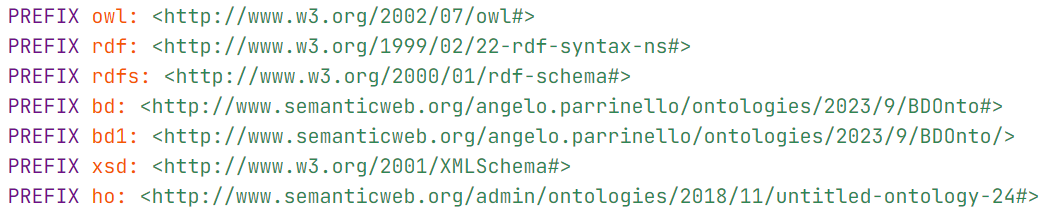
\includegraphics[width=15cm]{docs/images/prefix.PNG}
    \caption{Prefissi usati nelle query SPARQL.}
    \label{fig:prefix}
\end{figure}
In questa fase risulta di vitale importanza attivare il reasoner prima di lanciare qualunque query SPARQL all'interno di Protègè. Infatti il plugin per le query SPARQL di Protègè ha alcuni problemi tra cui alcuni legati all'UI: infatti se il reasoner è selezionato ma non attivo, alla richiesta di una query questo tornerà un risultato vuoto (si veda \cite{sparqluibug}).\\

Queste query sono state create usando \textbf{Protègè}, il suo plugin \textbf{Snap SPARQL Query} \cite{snapsparqlquery} e \textbf{GraphDB} \cite{graphdbhomepage}. In particolare, le query 2 e 6 sono state sviluppate e testate tramite GraphDB a causa di alcuni problemi legati a Protègè.
\newpage
\subsection{Query 1 - Tre Linugaggi più Popolari}
Questa query SPARQL consente di identificare i tre linguaggi di programmazione più supportati dal pool di strumenti big data presenti in questa ontologia. Le variabili \texttt{?language} e \texttt{?supportCount} vengono utilizzate per selezionare e contare, rispettivamente. Nella clausola \texttt{WHERE}, si devono rispettare certe condizioni: le variabili devono essere del tipo corretto e deve esistere una relazione tra di loro. La clausola \texttt{GROUP BY} raggruppa i risultati in base a \texttt{?language} che poi vengono ordinati in modo decrescente in base al numero di strumenti che supportano ciascun linguaggio. Infine, \texttt{LIMIT 3} limita i risultati alle prime tre occorrenze. Di seguito la query SPARQL prodotta.\\

\begin{lstlisting}[language=SQL]
SELECT ?language (COUNT(?tool) AS ?supportCount)
WHERE {
  ?language rdf:type bd:Programming_Language.
  ?tool rdf:type bd:Big_Data_Tool.  
  ?language bd:supportedBy ?tool.
}
GROUP BY ?language
ORDER BY DESC(?supportCount)
LIMIT 3
\end{lstlisting}


\subsection{Query 2 - Tecnologie non più supportate}
La seguente query SPARQL seleziona le tecnologie per i Big Data senza più supporto confrontando la data di fine del supporto di ciascuno strumento con la data attuale. Recupera le variabili \texttt{?tool, ?endDate} e \texttt{?currentDate}, filtra le istanze della classe corretta, recupera la data di fine supporto, ricava l'istante attuale con la funzione \texttt{NOW()} (che ritorna un tipo \texttt{xsd:dateTime} quindi direttamente confrontabile con le nostre date tramite l'operatore \texttt{<}) ed infine filtra solo gli strumenti la cui data di fine del supporto è precedente alla data attuale. I risultati sono ordinati in base alla data di fine del supporto in ordine ascendente. Di seguito la query finale.\\
\newpage
\begin{lstlisting}[language=SQL]
SELECT ?tool ?endDate ?currentDate
WHERE {
  ?tool rdf:type bd:Big_Data_Technology.
  ?tool bd:hasEndOfSupportDate ?endDate.
  BIND(NOW() AS ?currentDate)
  FILTER (?endDate < ?currentDate)
}
ORDER BY ASC(?endDate)
\end{lstlisting}
\subsection{Query 3 - Numero di Tool impiegati negli step di 'Data Visualization'}
L'intenzione di questa query SPARQL è estrarre informazioni sul numero di tool usati in ogni step di tipo \textit{Data\_Visualization}, tramite le operazione ad esso associate. Sapendo che ogni istanza di \textit{Data\_Visualization} è associata ad una operazione e che quest'ultima è associata a sua volta ad un tool, arriviamo a contare il numero univoco di istanze di \textit{Big\_Data\_Tool} collegate. Di seguito la query SPARQL creata.\\

\begin{lstlisting}[language=SQL]
SELECT ?tool (COUNT(DISTINCT ?dataVisualization) AS ?toolCount)
WHERE {
  ?dataVisualization rdf:type bd:Data_Visualization.
  ?dataVisualization bd:consistsOf ?operation.
  ?operation rdf:type bd:Operation.
  ?operation bd:hasParticipant ?tool.
}
GROUP BY ?tool
ORDER BY DESC(?toolCount)
\end{lstlisting}
\newpage
\subsection{Query 4 - Tre Tool con il tempo di supporto più lungo}
Prima di lanciare questa query è importante inferire l'informazione contenuta in \texttt{hasLifespan} (seguendo il percorso definito in \ref{subsec:premswrl}). La query filtra le istanze di tipo \texttt{Big\_Data\_Technology} e ne recupera il valore di \texttt{hasLifespan}. Infine, recupera le 3 tecnologie big data con il tempo di supporto più lungo, ordinando le istanze in modo decrescente sulla base dei tempi.\\

\begin{lstlisting}[language=SQL]
SELECT ?technology ?lifespan
WHERE {
  ?technology rdf:type bd:Big_Data_Technology.
  ?technology bd:hasLifespan ?lifespan.
}
ORDER BY DESC(?lifespan)
LIMIT 3
\end{lstlisting}

\subsection{Query 5 - Tecnologie con almeno la versione 3 e che sono tutt'ora supportate}
La seguente query SPARQL elenca le tecnologie che sono arrivati ad almeno la terza versione e che tale versione è supportata. Dopo aver selezionato le tecnologie, la propria versione ed eventualmente il nome completo (notare la clausola \texttt{OPTIONAL} che permette di includere le tecnologie che potrebbero non avere un nome completo, quindi non è una condizione vincolante), si cerca di recuperare anche la data di fine del supporto. Anche il recupero di tale campo risulta essere opzionale. L'operatore \texttt{bound} consente di verificare se una variabile è stata assegnata ad un valore. In questo specifico caso controlliamo se \texttt{endDate} è collegata alla tecnologia in questione o in altre parole controlliamo se l'istanza presa in considerazione ha associata una proprietà del tipo \texttt{hasEndOfSupportDate}. Quindi nella seconda \texttt{FILTER} filtriamo quelle tecnologie che o non hanno una data di fine supporto (e quindi assumiamo che siano ancora supportate) oppure tale data è antecedente al momento corrente. La seconda clausola di filtering  è importante che sia opzionale. Infatti, tale blocco rende la condizione sulla data di fine del supporto non vincolante per l'inclusione di una tecnologia nella risultante e quindi, se una tecnologia non ha una data di fine del supporto, viene comunque inclusa nella risultante. Infine, le istanze rimanenti vengono nuovamente filtrare in base al numero di versione. Di seguito la query creata.
\newpage
\begin{lstlisting}[language=SQL]
SELECT ?technology ?version ?fullName ?endDate
WHERE {
  ?technology rdf:type bd:Big_Data_Technology.
  ?technology bd:hasVersion ?version.
  OPTIONAL {?technology bd:hasFullName ?fullName.}
  OPTIONAL {
    ?technology bd:hasEndOfSupportDate ?endDate.
    BIND(NOW() AS ?currentDate)
    FILTER (!bound(?endDate) || ?endDate > ?currentDate)
  }
  FILTER (?version >= "3.0.0")
}
\end{lstlisting}

\subsection{Query 6 - Server supportati da AWS con almeno 16GB di RAM ed una GPU}
La seguente query evidenzia gli individui della classe Server, supportati dal servizio AWS e con almeno 16GB di RAM ed una GPU. Di seguito la query svluppata. Da notare la clausola \texttt{OPTIONAL} che controllo che almeno una proprietà legata alla GPU sia presente per definire o meno la presenza della stessa.
\begin{lstlisting}[language=SQL]
SELECT ?server
WHERE {
    ?server rdf:type bd1:Server.
    ?awsService rdf:type bd1:AWS.
    ?awsService bd:supportsWith ?server.
    
    ?server ho:deviceRAMUnit "GB"^^xsd:string.
    ?server ho:deviceRAMValue ?ramValue.
    FILTER(?ramValue >= 16)
    
    OPTIONAL {
        ?server ho:gpuMemoryUnit ?gpuMemoryUnit.
        ?server ho:gpuMemorySize ?gpuMemorySize.
        ?server ho:hasGPU ?hasGPU.
        FILTER (bound(?gpuMemoryUnit) || bound(?gpuMemorySize) || bound(?hasGPU) )
    }
}
\end{lstlisting}